
        \documentclass[12p]{article}
        \usepackage[margin=1in, left=1.5in, includefoot]{geometry}
        \usepackage{longtable, tabu}
        \usepackage[table, dvipsnames]{xcolor}
        \usepackage{array,booktabs}
        \usepackage{color}
        \usepackage{indentfirst}
        \usepackage{graphicx}
        \usepackage{float}
        \usepackage[utf8]{inputenc}
        \usepackage{listings}
        \usepackage{url}
        \usepackage{multirow}
        \usepackage{seqsplit}
        
        \definecolor{ferrarired}{rgb}{1.0, 0.11, 0.0}
        \definecolor{orange(colorwheel)}{rgb}{1.0, 0.5, 0.0}
        \definecolor{deepskyblue}{rgb}{0.0, 0.75, 1.0}
        \definecolor{grannysmithapple}{rgb}{0.66, 0.89, 0.63}
        \definecolor{gray(x11gray)}{rgb}{0.75, 0.75, 0.75}
        \definecolor{amber}{rgb}{1.0, 0.75, 0.0}
        
        \newcommand{\icon}[1]{\includegraphics[height=12pt]{#1}}
        \newcommand{\hash}[1]{{\ttfamily\seqsplit{#1}}}

        \setlength{\arrayrulewidth}{0.3mm}
\setlength{\tabcolsep}{18pt}
\renewcommand{\arraystretch}{1.5}
\setlength{\parindent}{1em}
\begin{document}
\begin{titlepage}
\begin{center}
\line(1,0){320}\\
[0.25in]
\huge{\bfseries Android Analysis Report}
\line(1,0){320}\\
[0.5in]
\begin{figure}[H]
	\centering
	
\includegraphics[scale=0.5]{/home/miki/Documents/GITHUB/AndroidPermissions/python/vulns/report_icons/logo.png}
\end{figure}
\textsl{\LARGE Demo app}\\
\textsf{\LARGE com.grppl.android.shell.halifax}\\
[2.5in]
\end{center}
\begin{flushright}
\textbf{\large Date 2018-06-14}
\end{flushright}
\end{titlepage}
\tableofcontents
\thispagestyle{empty}
\cleardoublepage
\setcounter{page}{1}
\section{PERMISSIONS}
	\begin{longtable}{p{3cm} p{10cm} }
	\rowcolor{grannysmithapple!70} Type & List \\
Normal &  ACCESS\_NETWORK\_STATE \\ 
 &  INSTALL\_SHORTCUT \\ 
 &  INSTALL\_SHORTCUT \\ 
\hline
Dangerous &  CAMERA \\ 
 &  ACCESS\_COARSE\_LOCATION \\ 
 &  ACCESS\_FINE\_LOCATION \\ 
 &  WRITE\_EXTERNAL\_STORAGE \\ 
\hline
Overprivileged &  USE\_FINGERPRINT \\ 
 &  READ\_EXTERNAL\_STORAGE \\ 
 &  READ\_CONTACTS \\ 
 &  RECEIVE\_BOOT\_COMPLETED \\ 
 &  INTERNET \\ 
 &  ACCESS\_WIFI\_STATE \\ 
 &  CALL\_PHONE \\ 
\hline
Underprivileged &  "android.permission.ACCESS\_COARSE\_LOCATION" \\ 
 &  UPDATE\_DEVICE\_STATS \\ 
 &  ACCESS\_COARSE\_LOCATION \\ 
 &  "android.permission.ACCESS\_NETWORK\_STATE" \\ 
 &  INSTALL\_SHORTCUT \\ 
 &  "android.permission.ACCESS\_FINE\_LOCATION" \\ 
\hline
Automatically granted dangerous permissions &  WRITE\_CONTACTS \\ 
 &  GET\_ACCOUNTS \\ 
 &  ANSWER\_PHONE\_CALLSREAD\_PHONE\_NUMBERS \\ 
 &  READ\_PHONE\_STATE \\ 
 &  READ\_CALL\_LOG \\ 
 &  WRITE\_CALL\_LOG \\ 
 &  ADD\_VOICEMAIL \\ 
 &  USE\_SIP \\ 
 &  PROCESS\_OUTGOING\_CALLS \\ 
\hline
	\end{longtable}
\section{FINDINGS SUMMARY}\label{sec:summary}
\begin{figure}[H]
\centering
	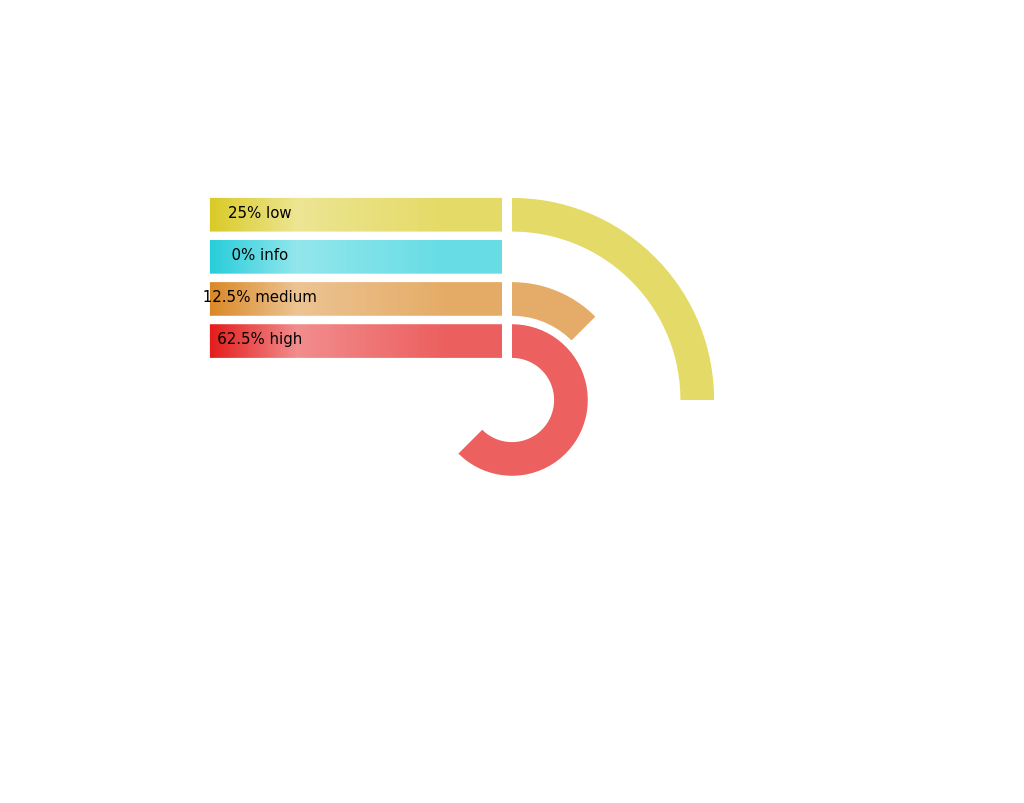
\includegraphics[scale=0.5]{/home/miki/Documents/GITHUB/AndroidPermissions/apks/playstore_apps/com_grppl_android_shell_halifax/report/pie_chart.png}
\end{figure}
	\begin{longtable}{p{0.5cm} p{10cm} p{1.5cm}}
	\rowcolor{grannysmithapple!70} Index & Title & Impact \\
	A1&& \color{amber}\textbf{Low} \\
\hline\\	A2&JavascriptInterfaceAnalyser& \color{ferrarired}\textbf{High} \\
\hline\\	A3&Electronic Codebook \newline (ECB) used for encryption& \color{ferrarired}\textbf{High} \\
\hline\\	A4&Activity \newline (com. halifax. halifax. GrappleActivity) is not Protected. An intent-filter exists.& \color{ferrarired}\textbf{High} \\
\hline\\	A5&Launch Mode of Activity \newline (com. mobile. ui. webjourney. activity. AuthWebJourneyActivity) is not standard.& \color{ferrarired}\textbf{High} \\
\hline\\	A6&Launch Mode of Activity \newline (com. mobile. ui. home. activity. YourAccountsActivity) is not standard.& \color{ferrarired}\textbf{High} \\
\hline\\	A7&Launch Mode of Activity \newline (com. mobile. ui. settings. activity. SecuritySettingsActivity) is not standard.& \color{ferrarired}\textbf{High} \\
\hline\\	A8&Launch Mode of Activity \newline (com. mobile. ui. settings. activity. PersonalDetailsSettingsActivity) is not standard.& \color{ferrarired}\textbf{High} \\
\hline\\	A9&Launch Mode of Activity \newline (com. mobile. ui. settings. activity. SettingsAndInfoActivity) is not standard.& \color{ferrarired}\textbf{High} \\
\hline\\	A10&Launch Mode of Activity \newline (com. mobile. ui. producthub. activity. ProductHubActivity) is not standard.& \color{ferrarired}\textbf{High} \\
\hline\\	A11&Launch Mode of Activity \newline (com. mobile. ui. mobilechat. activity. MobileChatActivity) is not standard.& \color{ferrarired}\textbf{High} \\
\hline\\	A12&Launch Mode of Activity \newline (com. mobile. ui. branchfinder. activity. BranchFinderActivity) is not standard.& \color{ferrarired}\textbf{High} \\
\hline\\	A13&Launch Mode of Activity \newline (com. mobile. ui. unsuretransaction. activity. UnsureTransactionActivity) is not standard.& \color{ferrarired}\textbf{High} \\
\hline\\	A14&Launch Mode of Activity \newline (com. liveperson. infra. messaging\_ ui. ConversationActivity) is not standard.& \color{ferrarired}\textbf{High} \\
\hline\\	A15&& \color{amber}\textbf{Low} \\
\hline\\	\end{longtable}
\cleardoublepage
\newpage
\section{DETAILED FINDINGS}
\subsection{A1: }
\subsubsection*{\protect\icon{/home/miki/Documents/GITHUB/AndroidPermissions/python/vulns/report_icons/basic_sheet.png} Description}

\subsubsection*{\protect\icon{/home/miki/Documents/GITHUB/AndroidPermissions/python/vulns/report_icons/basic_magnifier.png} Evidence}
\path{/home/miki/Documents/GITHUB/AndroidPermissions/apks/playstore_apps/com_grppl_android_shell_halifax/app/smali/android/support/v4/text/ICUCompatIcs.smali
Landroid/util/Log -> w(Ljava/lang/String;Ljava/lang/Throwable;)}

\path{/home/miki/Documents/GITHUB/AndroidPermissions/apks/playstore_apps/com_grppl_android_shell_halifax/app/smali/android/support/v4/text/ICUCompatIcs.smali
Landroid/util/Log -> w(Ljava/lang/String;Ljava/lang/Throwable;)}

\path{/home/miki/Documents/GITHUB/AndroidPermissions/apks/playstore_apps/com_grppl_android_shell_halifax/app/smali/android/support/v4/text/ICUCompatIcs.smali
Landroid/util/Log -> w(Ljava/lang/String;Ljava/lang/Throwable;)}

\path{/home/miki/Documents/GITHUB/AndroidPermissions/apks/playstore_apps/com_grppl_android_shell_halifax/app/smali/android/support/v4/text/ICUCompatIcs.smali
Landroid/util/Log -> w(Ljava/lang/String;Ljava/lang/Throwable;)}

\path{/home/miki/Documents/GITHUB/AndroidPermissions/apks/playstore_apps/com_grppl_android_shell_halifax/app/smali/android/support/v4/text/ICUCompatIcs.smali
Landroid/util/Log -> w(Ljava/lang/String;Ljava/lang/Throwable;)}

\path{/home/miki/Documents/GITHUB/AndroidPermissions/apks/playstore_apps/com_grppl_android_shell_halifax/app/smali/android/support/v4/text/ICUCompatApi21.smali
Landroid/util/Log -> w(Ljava/lang/String;Ljava/lang/Throwable;)}

\path{/home/miki/Documents/GITHUB/AndroidPermissions/apks/playstore_apps/com_grppl_android_shell_halifax/app/smali/android/support/v4/text/ICUCompatApi21.smali
Landroid/util/Log -> w(Ljava/lang/String;Ljava/lang/Throwable;)}

\path{/home/miki/Documents/GITHUB/AndroidPermissions/apks/playstore_apps/com_grppl_android_shell_halifax/app/smali/android/support/v4/print/PrintHelper$PrintHelperApi19$2.smali
Landroid/util/Log -> e(Ljava/lang/String;Ljava/lang/String;Ljava/lang/Throwable;)}

\path{/home/miki/Documents/GITHUB/AndroidPermissions/apks/playstore_apps/com_grppl_android_shell_halifax/app/smali/android/support/v4/print/PrintHelper$PrintHelperApi19.smali
Landroid/util/Log -> w(Ljava/lang/String;Ljava/lang/String;Ljava/lang/Throwable;)}

\path{/home/miki/Documents/GITHUB/AndroidPermissions/apks/playstore_apps/com_grppl_android_shell_halifax/app/smali/android/support/v4/print/PrintHelper$PrintHelperApi19.smali
Landroid/util/Log -> w(Ljava/lang/String;Ljava/lang/String;Ljava/lang/Throwable;)}


\textit{snip}
\newline \textsl{For the full list view \path{/home/miki/Documents/GITHUB/AndroidPermissions/apks/playstore_apps/com_grppl_android_shell_halifax/report}}
\subsubsection*{\protect\icon{/home/miki/Documents/GITHUB/AndroidPermissions/python/vulns/report_icons/basic_todo.png} Recommendation}

\subsection{A2: JavascriptInterfaceAnalyser}
\subsubsection*{\protect\icon{/home/miki/Documents/GITHUB/AndroidPermissions/python/vulns/report_icons/basic_sheet.png} Description}

\subsubsection*{\protect\icon{/home/miki/Documents/GITHUB/AndroidPermissions/python/vulns/report_icons/basic_magnifier.png} Evidence}
\path{/home/miki/Documents/GITHUB/AndroidPermissions/apks/playstore_apps/com_grppl_android_shell_halifax/app/smali/com/mobile/ui/common/view/SecureCoreWebView.smali addJavascriptInterface}

\subsubsection*{\protect\icon{/home/miki/Documents/GITHUB/AndroidPermissions/python/vulns/report_icons/basic_todo.png} Recommendation}

\subsection{A3: Electronic Codebook (ECB) used for encryption}
\subsubsection*{\protect\icon{/home/miki/Documents/GITHUB/AndroidPermissions/python/vulns/report_icons/basic_sheet.png} Description}

            Using the same encryption key, in ECB mode data blocks are enciphered individually 
            from each other and cause identical message blocks to be transformed to identical ciphertext 
            blocks. The independency of encrypted blocks also implies that the malicious substitution of a 
            block has no impact on adjacent blocks. As a consequence, data patterns are not well hidden and 
            message confidentiality may be compromised.
            
            On Android, the Cipher API provides access to implementations of cryptographic schemes
            for the encryption and decryption of arbitrary data. To request an instance of a particular cipher,
            an application has to invoke the method getInstance, passing a suitable transformation string as
            parameter. Typically, this value is composed of the desired algorithm name, a mode of operation,
            and the padding scheme to apply. For example, to request an object instance that provides AES in
            ECB mode with PKCS5 padding, the transformation AES/ECB/PKCS5Padding has to be specified.
            
            While it is indispensable to declare the algorithm to use, explicitly setting the mode and
            padding may be omitted. To fill the gap, the underlying Cryptographic Service Provider (CSP)
            relies on predefined values that do not necessarily reflect the recommended practice. Precisely, if
            the transformation indicates no operation mode, ECB mode is put in place. Moreover, the initially
            described problem with ECB is not limited to a specific cipher, such as AES but affects all symmetric
            block ciphers. Stream ciphers and asymmetric cryptosystems are not concerned since they
            do not involve an operation mode to repeatedly encipher blocks of contiguous data.
        
\subsubsection*{\protect\icon{/home/miki/Documents/GITHUB/AndroidPermissions/python/vulns/report_icons/basic_magnifier.png} Evidence}
\path{/home/miki/Documents/GITHUB/AndroidPermissions/apks/playstore_apps/com_grppl_android_shell_halifax/app/smali/kkkkkk/knnnkk.smali}

\path{/home/miki/Documents/GITHUB/AndroidPermissions/apks/playstore_apps/com_grppl_android_shell_halifax/app/smali/kkkkkk/dxxdxx.smali}

\path{/home/miki/Documents/GITHUB/AndroidPermissions/apks/playstore_apps/com_grppl_android_shell_halifax/app/smali/kkkkkk/dxxdxx.smali}

\path{/home/miki/Documents/GITHUB/AndroidPermissions/apks/playstore_apps/com_grppl_android_shell_halifax/app/smali/kkkkkk/dxxdxx.smali}

\path{/home/miki/Documents/GITHUB/AndroidPermissions/apks/playstore_apps/com_grppl_android_shell_halifax/app/smali/kkkkkk/dxxdxx.smali}

\subsubsection*{\protect\icon{/home/miki/Documents/GITHUB/AndroidPermissions/python/vulns/report_icons/basic_todo.png} Recommendation}
It is recommended not to use ECB for encryption. Use an asymmetric encryption algorithm instead
\subsection{A4: Activity (com. halifax. halifax. GrappleActivity) is not Protected. An intent-filter exists.}
\subsubsection*{\protect\icon{/home/miki/Documents/GITHUB/AndroidPermissions/python/vulns/report_icons/basic_sheet.png} Description}
A  Activity is found to be shared with other apps on the device therefore leaving it accessible to any other application on the device. The presence of intent-filter indicates that the Activity is explicitly exported.
\subsubsection*{\protect\icon{/home/miki/Documents/GITHUB/AndroidPermissions/python/vulns/report_icons/basic_todo.png} Recommendation}
It is recommended to set the protection level to signature, so only applications signed with the same certificate can obtain the permission.
\subsection{A5: Launch Mode of Activity (com. mobile. ui. webjourney. activity. AuthWebJourneyActivity) is not standard.}
\subsubsection*{\protect\icon{/home/miki/Documents/GITHUB/AndroidPermissions/python/vulns/report_icons/basic_sheet.png} Description}
An Activity should not be having the launch mode attribute set to "singleTask/singleInstance" as it becomes root Activity and it is possible for other applications to read the contents of the calling Intent.
\subsubsection*{\protect\icon{/home/miki/Documents/GITHUB/AndroidPermissions/python/vulns/report_icons/basic_todo.png} Recommendation}
It is required to use the "standard" launch mode attribute when sensitive information is included in an Intent.
\subsection{A6: Launch Mode of Activity (com. mobile. ui. home. activity. YourAccountsActivity) is not standard.}
\subsubsection*{\protect\icon{/home/miki/Documents/GITHUB/AndroidPermissions/python/vulns/report_icons/basic_sheet.png} Description}
An Activity should not be having the launch mode attribute set to "singleTask/singleInstance" as it becomes root Activity and it is possible for other applications to read the contents of the calling Intent.
\subsubsection*{\protect\icon{/home/miki/Documents/GITHUB/AndroidPermissions/python/vulns/report_icons/basic_todo.png} Recommendation}
It is required to use the "standard" launch mode attribute when sensitive information is included in an Intent.
\subsection{A7: Launch Mode of Activity (com. mobile. ui. settings. activity. SecuritySettingsActivity) is not standard.}
\subsubsection*{\protect\icon{/home/miki/Documents/GITHUB/AndroidPermissions/python/vulns/report_icons/basic_sheet.png} Description}
An Activity should not be having the launch mode attribute set to "singleTask/singleInstance" as it becomes root Activity and it is possible for other applications to read the contents of the calling Intent.
\subsubsection*{\protect\icon{/home/miki/Documents/GITHUB/AndroidPermissions/python/vulns/report_icons/basic_todo.png} Recommendation}
It is required to use the "standard" launch mode attribute when sensitive information is included in an Intent.
\subsection{A8: Launch Mode of Activity (com. mobile. ui. settings. activity. PersonalDetailsSettingsActivity) is not standard.}
\subsubsection*{\protect\icon{/home/miki/Documents/GITHUB/AndroidPermissions/python/vulns/report_icons/basic_sheet.png} Description}
An Activity should not be having the launch mode attribute set to "singleTask/singleInstance" as it becomes root Activity and it is possible for other applications to read the contents of the calling Intent.
\subsubsection*{\protect\icon{/home/miki/Documents/GITHUB/AndroidPermissions/python/vulns/report_icons/basic_todo.png} Recommendation}
It is required to use the "standard" launch mode attribute when sensitive information is included in an Intent.
\subsection{A9: Launch Mode of Activity (com. mobile. ui. settings. activity. SettingsAndInfoActivity) is not standard.}
\subsubsection*{\protect\icon{/home/miki/Documents/GITHUB/AndroidPermissions/python/vulns/report_icons/basic_sheet.png} Description}
An Activity should not be having the launch mode attribute set to "singleTask/singleInstance" as it becomes root Activity and it is possible for other applications to read the contents of the calling Intent.
\subsubsection*{\protect\icon{/home/miki/Documents/GITHUB/AndroidPermissions/python/vulns/report_icons/basic_todo.png} Recommendation}
It is required to use the "standard" launch mode attribute when sensitive information is included in an Intent.
\subsection{A10: Launch Mode of Activity (com. mobile. ui. producthub. activity. ProductHubActivity) is not standard.}
\subsubsection*{\protect\icon{/home/miki/Documents/GITHUB/AndroidPermissions/python/vulns/report_icons/basic_sheet.png} Description}
An Activity should not be having the launch mode attribute set to "singleTask/singleInstance" as it becomes root Activity and it is possible for other applications to read the contents of the calling Intent.
\subsubsection*{\protect\icon{/home/miki/Documents/GITHUB/AndroidPermissions/python/vulns/report_icons/basic_todo.png} Recommendation}
It is required to use the "standard" launch mode attribute when sensitive information is included in an Intent.
\subsection{A11: Launch Mode of Activity (com. mobile. ui. mobilechat. activity. MobileChatActivity) is not standard.}
\subsubsection*{\protect\icon{/home/miki/Documents/GITHUB/AndroidPermissions/python/vulns/report_icons/basic_sheet.png} Description}
An Activity should not be having the launch mode attribute set to "singleTask/singleInstance" as it becomes root Activity and it is possible for other applications to read the contents of the calling Intent.
\subsubsection*{\protect\icon{/home/miki/Documents/GITHUB/AndroidPermissions/python/vulns/report_icons/basic_todo.png} Recommendation}
It is required to use the "standard" launch mode attribute when sensitive information is included in an Intent.
\subsection{A12: Launch Mode of Activity (com. mobile. ui. branchfinder. activity. BranchFinderActivity) is not standard.}
\subsubsection*{\protect\icon{/home/miki/Documents/GITHUB/AndroidPermissions/python/vulns/report_icons/basic_sheet.png} Description}
An Activity should not be having the launch mode attribute set to "singleTask/singleInstance" as it becomes root Activity and it is possible for other applications to read the contents of the calling Intent.
\subsubsection*{\protect\icon{/home/miki/Documents/GITHUB/AndroidPermissions/python/vulns/report_icons/basic_todo.png} Recommendation}
It is required to use the "standard" launch mode attribute when sensitive information is included in an Intent.
\subsection{A13: Launch Mode of Activity (com. mobile. ui. unsuretransaction. activity. UnsureTransactionActivity) is not standard.}
\subsubsection*{\protect\icon{/home/miki/Documents/GITHUB/AndroidPermissions/python/vulns/report_icons/basic_sheet.png} Description}
An Activity should not be having the launch mode attribute set to "singleTask/singleInstance" as it becomes root Activity and it is possible for other applications to read the contents of the calling Intent.
\subsubsection*{\protect\icon{/home/miki/Documents/GITHUB/AndroidPermissions/python/vulns/report_icons/basic_todo.png} Recommendation}
It is required to use the "standard" launch mode attribute when sensitive information is included in an Intent.
\subsection{A14: Launch Mode of Activity (com. liveperson. infra. messaging\_ ui. ConversationActivity) is not standard.}
\subsubsection*{\protect\icon{/home/miki/Documents/GITHUB/AndroidPermissions/python/vulns/report_icons/basic_sheet.png} Description}
An Activity should not be having the launch mode attribute set to "singleTask/singleInstance" as it becomes root Activity and it is possible for other applications to read the contents of the calling Intent.
\subsubsection*{\protect\icon{/home/miki/Documents/GITHUB/AndroidPermissions/python/vulns/report_icons/basic_todo.png} Recommendation}
It is required to use the "standard" launch mode attribute when sensitive information is included in an Intent.
\subsection{A15: }
\subsubsection*{\protect\icon{/home/miki/Documents/GITHUB/AndroidPermissions/python/vulns/report_icons/basic_sheet.png} Description}

\subsubsection*{\protect\icon{/home/miki/Documents/GITHUB/AndroidPermissions/python/vulns/report_icons/basic_magnifier.png} Evidence}
\path{/home/miki/Documents/GITHUB/AndroidPermissions/apks/playstore_apps/com_grppl_android_shell_halifax/app/smali/android/arch/lifecycle/Lifecycling.smali forName}

\path{/home/miki/Documents/GITHUB/AndroidPermissions/apks/playstore_apps/com_grppl_android_shell_halifax/app/smali/android/arch/lifecycle/ReflectiveGenericLifecycleObserver.smali getSuperclass}

\path{/home/miki/Documents/GITHUB/AndroidPermissions/apks/playstore_apps/com_grppl_android_shell_halifax/app/smali/android/arch/lifecycle/ReflectiveGenericLifecycleObserver.smali invoke}

\path{/home/miki/Documents/GITHUB/AndroidPermissions/apks/playstore_apps/com_grppl_android_shell_halifax/app/smali/android/support/v4/text/ICUCompatIcs.smali forName}

\path{/home/miki/Documents/GITHUB/AndroidPermissions/apks/playstore_apps/com_grppl_android_shell_halifax/app/smali/android/support/v4/text/ICUCompatIcs.smali invoke}

\path{/home/miki/Documents/GITHUB/AndroidPermissions/apks/playstore_apps/com_grppl_android_shell_halifax/app/smali/android/support/v4/text/ICUCompatIcs.smali invoke}

\path{/home/miki/Documents/GITHUB/AndroidPermissions/apks/playstore_apps/com_grppl_android_shell_halifax/app/smali/android/support/v4/text/ICUCompatApi21.smali forName}

\path{/home/miki/Documents/GITHUB/AndroidPermissions/apks/playstore_apps/com_grppl_android_shell_halifax/app/smali/android/support/v4/text/ICUCompatApi21.smali invoke}

\path{/home/miki/Documents/GITHUB/AndroidPermissions/apks/playstore_apps/com_grppl_android_shell_halifax/app/smali/android/support/v4/util/ArraySet.smali getComponentType}

\path{/home/miki/Documents/GITHUB/AndroidPermissions/apks/playstore_apps/com_grppl_android_shell_halifax/app/smali/android/support/v4/util/MapCollections.smali getComponentType}


\textit{snip}
\newline \textsl{For the full list view \path{/home/miki/Documents/GITHUB/AndroidPermissions/apks/playstore_apps/com_grppl_android_shell_halifax/report}}
\subsubsection*{\protect\icon{/home/miki/Documents/GITHUB/AndroidPermissions/python/vulns/report_icons/basic_todo.png} Recommendation}

\cleardoublepage
\newpage
\section{VISUALIZATIONS}
\subsection{Chord Diagram - Class Relations}
\begin{figure}[H]
	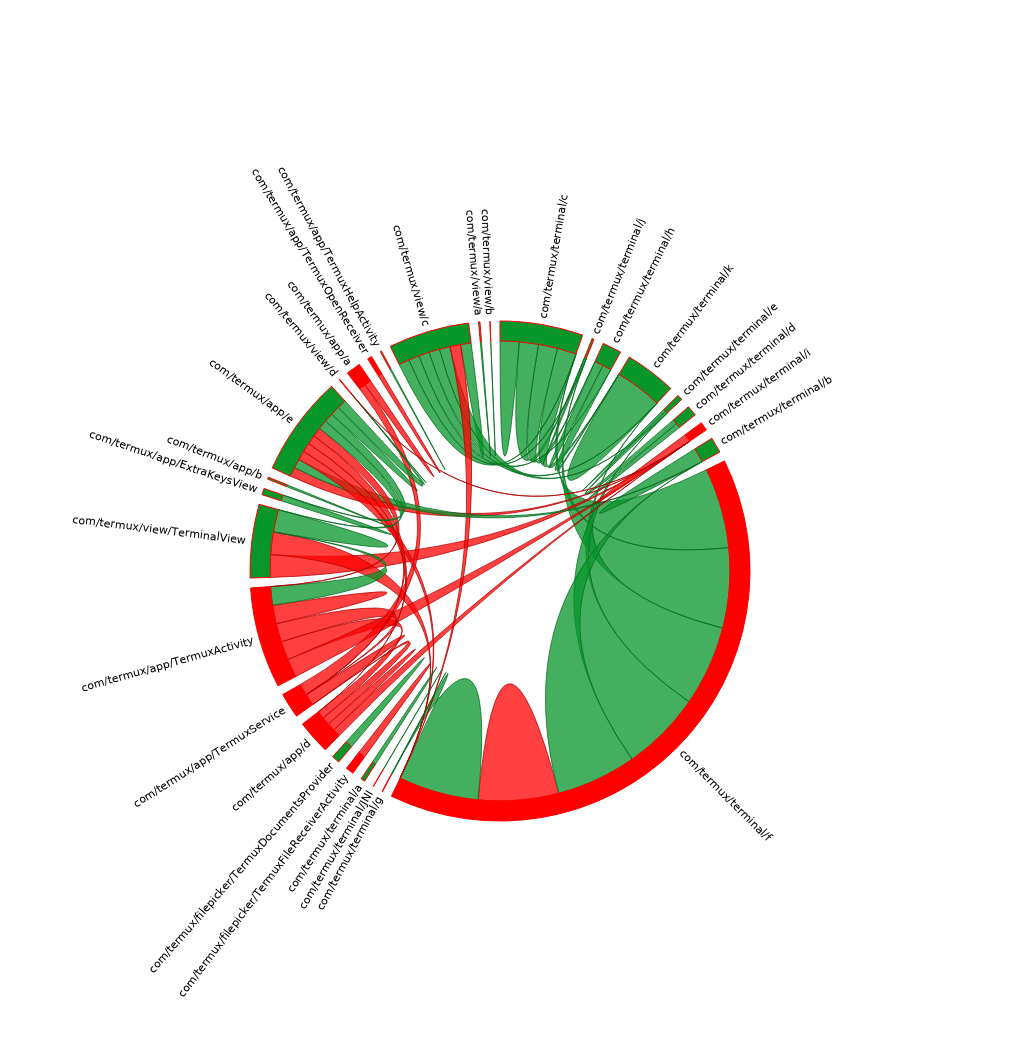
\includegraphics[scale=0.45]{/home/miki/Documents/GITHUB/AndroidPermissions/apks/playstore_apps/com_grppl_android_shell_halifax/report/chord_diagram.png}\end{figure}\subsection{Hot Spot - System Overview}
\begin{figure}[H]
\centering
	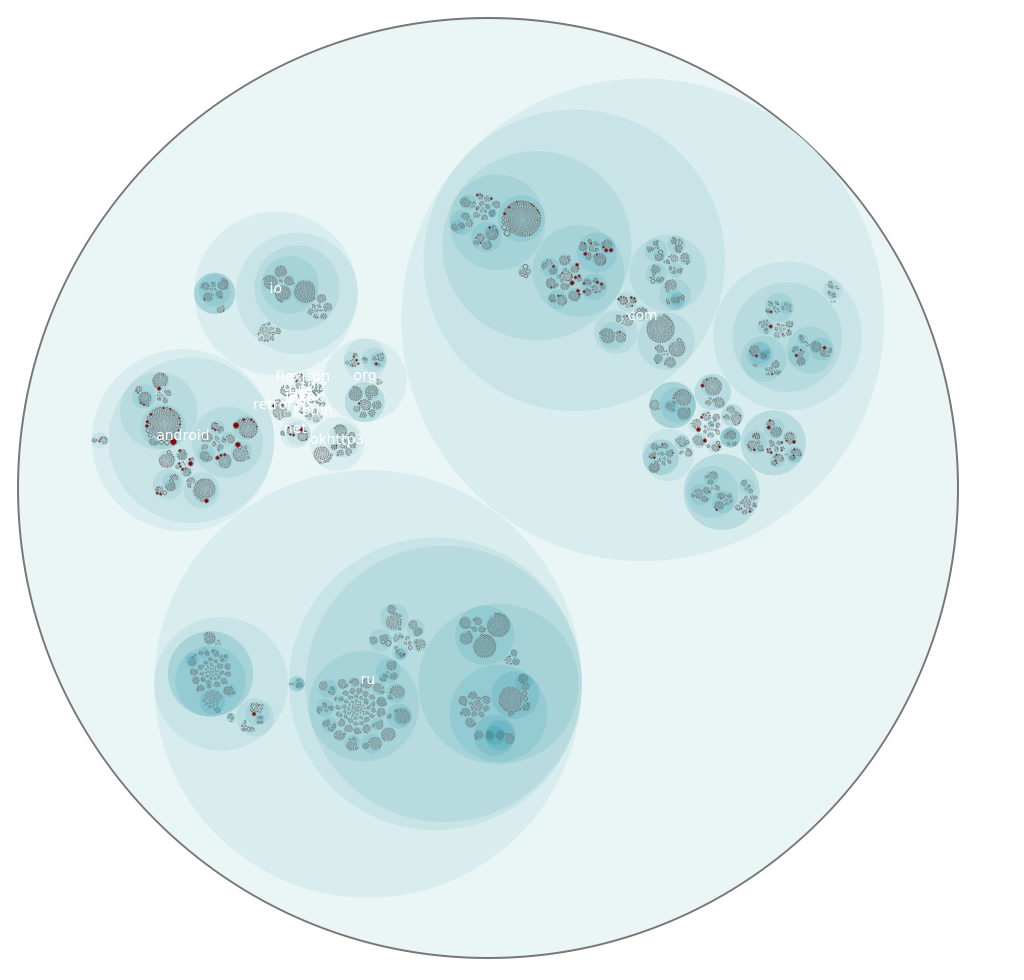
\includegraphics[scale=0.5]{/home/miki/Documents/GITHUB/AndroidPermissions/apks/playstore_apps/com_grppl_android_shell_halifax/report/hotspot.png}\end{figure}\begin{longtable}{p{0.3cm} p{12cm}}
\rowcolor{orange} Index & Class \\
1 & \path{/home/miki/Documents/GITHUB/AndroidPermissions/apks/playstore_apps/com_grppl_android_shell_halifax/app/smali/com/topimagesystems/controllers/imageanalyze/CameraController.smali} \\
2 & \path{/home/miki/Documents/GITHUB/AndroidPermissions/apks/playstore_apps/com_grppl_android_shell_halifax/app/smali/com/topimagesystems/controllers/imageanalyze/CameraController$CameraActivityHandler.smali} \\
3 & \path{/home/miki/Documents/GITHUB/AndroidPermissions/apks/playstore_apps/com_grppl_android_shell_halifax/app/smali/com/topimagesystems/controllers/imageanalyze/CameraSessionManager.smali} \\
4 & \path{/home/miki/Documents/GITHUB/AndroidPermissions/apks/playstore_apps/com_grppl_android_shell_halifax/app/smali/android/support/multidex/MultiDex.smali} \\
5 & \path{/home/miki/Documents/GITHUB/AndroidPermissions/apks/playstore_apps/com_grppl_android_shell_halifax/app/smali/com/topimagesystems/util/FileUtils.smali} \\
6 & \path{/home/miki/Documents/GITHUB/AndroidPermissions/apks/playstore_apps/com_grppl_android_shell_halifax/app/smali/android/support/v4/media/MediaBrowserCompat$MediaBrowserImplBase.smali} \\
7 & \path{/home/miki/Documents/GITHUB/AndroidPermissions/apks/playstore_apps/com_grppl_android_shell_halifax/app/smali/android/support/v4/media/session/MediaControllerCompat$TransportControlsBase.smali} \\
8 & \path{/home/miki/Documents/GITHUB/AndroidPermissions/apks/playstore_apps/com_grppl_android_shell_halifax/app/smali/android/support/v4/media/session/MediaControllerCompat$MediaControllerImplBase.smali} \\
9 & \path{/home/miki/Documents/GITHUB/AndroidPermissions/apks/playstore_apps/com_grppl_android_shell_halifax/app/smali/android/support/multidex/MultiDexExtractor.smali} \\
10 & \path{/home/miki/Documents/GITHUB/AndroidPermissions/apks/playstore_apps/com_grppl_android_shell_halifax/app/smali/com/topimagesystems/controllers/imageanalyze/CameraManagerController.smali} \\
	\end{longtable}
\end{document}
